%%
%% Migrated manuscript: A.tex content merged into the ICT Express / Elsevier
%% cas-dc double-column template (B.tex).
%%
\documentclass[a4paper,fleqn]{cas-dc}

\usepackage[numbers]{natbib}

% ---------------------------------------------------------------------
% Additional packages required to reproduce the content of the original
% manuscript (equations, algorithms, tables, figures, citations).
% Only packages that are NOT already provided by cas-dc are added here,
% so that the layout, fonts, and structural rules of the template are
% preserved.
% ---------------------------------------------------------------------
\usepackage{amsmath,amssymb,amsfonts}
\usepackage{graphicx}
\usepackage{booktabs}
\usepackage{array}
\usepackage{multirow}
\usepackage{subcaption}
\usepackage{threeparttable}
\usepackage{bm}
\usepackage{makecell}
\usepackage{xurl}
\usepackage{xcolor}
\usepackage{tabularray}
\usepackage{csvsimple-l3}
\usepackage{algorithm}
\usepackage{algorithmicx}
\usepackage{algpseudocode}

\algdef{SE}[SUBALG]{Indent}{EndIndent}{}{\algorithmicend\ }
\algtext*{Indent}
\algtext*{EndIndent}
\algnewcommand\algorithmparam{\textbf{Parameters:}}
\algnewcommand\Param{\item[\algorithmparam]}
\renewcommand{\algorithmicrequire}{\textbf{Input:}}
\renewcommand{\algorithmicensure}{\textbf{Output:}}

%%%Author definitions
\def\tsc#1{\csdef{#1}{\textsc{\lowercase{#1}}\xspace}}
\tsc{DL}
\tsc{CCTV}
\tsc{FPS}
\tsc{FAR}
%%%

\begin{document}
	\let\WriteBookmarks\relax
	\def\floatpagepagefraction{1}
	\def\textpagefraction{.001}
	
	\shorttitle{Motion-Heuristic Skip Module for Real-Time Fire Surveillance}
	\shortauthors{Hoang Van-Ha et~al.}
	
	\title[mode=title]{Efficient Real-Time Fire Surveillance: A Lightweight
		Motion-Heuristic Skip Module for Accelerated Inference in Indoor
		Environments}
	
	\author[1]{Hoang Van-Ha}
	\cormark[1]
	\ead{}
	
	\author[1]{Jong Weon Lee}
	
	\author[1]{Park Chun-Su}
	\cormark[1]
	
	\affiliation[1]{organization={Sejong University},
		addressline={},
		city={Seoul},
		country={Republic of Korea}}
	
	\cortext[cor1]{Corresponding author}
	
	\begin{abstract}
		Conventional deep learning (DL)-based fire and smoke detection systems
		perform inference on every video frame using high-complexity models to
		classify the presence of fire or smoke. However, in surveillance
		scenarios, particularly indoor environments, video streams frequently
		contain long periods of static background frames with little or no
		motion, rendering per-frame inference redundant and wasteful of
		computational resources. To address this limitation, this study proposes
		an efficient inference acceleration framework for fire and smoke
		surveillance systems that combines a motion-aware skip module with an
		Eager mode for recall recovery. The skip module leverages motion
		detection to selectively bypass unnecessary DL inference on
		non-informative frames, while the Eager mode periodically forces
		inference updates to mitigate missed detections from slow-developing or
		nearly stationary smoke events. Evaluation on a large-scale dataset
		comprising 150 indoor videos demonstrates that the proposed framework
		achieves nearly 30\% higher throughput than the baseline performing
		per-frame inference, with only a 0.05\% reduction in recall. In
		contrast, using the skip module alone results in a 1.23\% recall drop,
		highlighting the effectiveness of the Eager mode in recovering detection
		performance while preserving most of the throughput gain. These results
		demonstrate that the proposed framework provides an effective
		plug-and-play inference acceleration strategy for real-time indoor fire
		and smoke surveillance systems.
	\end{abstract}
	
	\begin{keywords}
		Fire and smoke detection \sep motion-based skip module \sep inference
		acceleration \sep video surveillance \sep deep learning
	\end{keywords}
	
	\maketitle
	
	\section{Introduction}\label{sec:introduction}
	
	Fires and wildfires, if not detected and controlled in their early
	stages, can quickly escalate, especially under dry and windy conditions,
	resulting in catastrophic consequences, including loss of life,
	destruction of property, and damage to natural ecosystems. For instance,
	in 2017, urban fires and wildfires in California, USA, caused an
	estimated economic loss of 10 billion USD \citep{californiafire:online}.
	More recently, in 2025, a forest fire in Gyeongsang Province, South
	Korea, burned approximately 90,000 acres, resulting in at least 27
	fatalities and the evacuation of nearly 40,000 residents
	\citep{southkoreafire:online}. These incidents highlight the critical
	importance of automated early-stage fire and smoke detection systems for
	enabling timely intervention and minimizing damage.
	
	In recent years, DL-based approaches have emerged as the prevailing
	methodology in fire and smoke detection systems
	\citep{cheng2024visual,gragnaniello2024fire}. In practical deployments,
	such systems are commonly integrated into CCTV video pipelines, where
	DL-based classifiers or object detectors perform inference on every
	individual frame. While this per-frame paradigm is straightforward to
	implement, it exhibits two major limitations. First, it relies solely on
	spatial information within isolated frames, neglecting temporal cues
	like motion in video sequences. Second, in surveillance scenarios,
	particularly in \textbf{indoor} environments, video streams can exhibit
	minimal visual variation across consecutive frames due to static scene
	content. Indiscriminately applying computationally intensive DL models
	to every frame under these conditions introduces significant processing
	redundancy, increasing latency and computational overhead without
	improving detection performance. This inefficiency is further amplified
	by the well-known accuracy-efficiency trade-off in DL: high-accuracy
	models typically demand substantial computational resources, and
	indiscriminate per-frame inference magnifies these demands, posing a
	significant barrier to real-time deployment.
	
	A common strategy for reducing inference cost is to substitute a
	high-complexity model with a lightweight alternative; however, this
	approach typically compromises detection reliability --- an unacceptable
	trade-off in safety-critical applications such as fire and smoke
	surveillance. This study adopts a complementary approach: rather than
	replacing the classifier, we propose an efficient inference acceleration
	framework that introduces a lightweight, motion-aware skip module acting
	as a computational gate upstream of the classifier. The skip module
	leverages frame differencing-based motion estimation to selectively
	bypass DL inference on static, non-informative frames, while forwarding
	only frames with significant scene activity to the high-capacity
	classifier. To address a key failure mode of motion-based skipping ---
	namely, missed detections arising from slow-developing or nearly
	stationary smoke events --- the framework additionally incorporates an
	Eager mode that periodically forces inference updates to recover
	detection recall. As illustrated in Fig.~\ref{fig:pipeline}, the
	conventional pipeline processes every frame through the classifier,
	whereas the proposed pipeline adds the skip module early in the process
	to conditionally suppress redundant inference calls.
	
	In particular, our main contributions are summarized as follows:
	
	\begin{itemize}
		\item \textbf{Motion-Aware Skip Module:} A lightweight skip module is
		proposed that exploits frame differencing-based motion estimation to
		identify and bypass DL inference on static frames, thereby reducing
		computational cost without modifying the underlying classifier. The
		proposed module is designed as a plug-and-play component compatible
		with existing fire and smoke detection pipelines. A systematic
		hyperparameter optimization procedure is developed to identify the
		optimal operating configuration for maximizing throughput while
		preserving detection performance. The skip module is further augmented
		with \textsc{Eager} mode, which mitigates missed detections on
		slow-developing or nearly stationary smoke --- a key failure mode of
		motion-based skipping.
		\item \textbf{Indoor Fire and Smoke Video Dataset:} We construct an
		annotated dataset comprising 150 indoor fire and smoke videos
		(including fire, smoke, and background-only classes) captured by
		static surveillance cameras at resolutions ranging from
		$814 \times 720$ to $3840 \times 2160$. The dataset covers diverse
		environments such as warehouses, parking areas, and offices under
		varying lighting conditions, providing a realistic benchmark for
		evaluating detection systems in static surveillance scenarios.
		\item \textbf{Comprehensive System Evaluation and Analysis:} The
		proposed framework is integrated with a high-capacity DL classifier
		(BIG Model) and evaluated on the constructed dataset against a
		per-frame inference baseline and existing methods. Results demonstrate
		approximately 30\% higher throughput than the baseline, with a recall
		reduction of roughly 0.05\% when the Eager mode is active --- compared
		to a 1.23\% recall drop when the skip module is used alone ---
		highlighting the effectiveness of the Eager mode in recovering
		detection performance while preserving most throughput gains. Beyond
		quantitative benchmarking, a detailed efficiency analysis of the
		proposed system is conducted, alongside a qualitative examination of
		representative success and failure cases.
	\end{itemize}
	
	The rest of this paper is organized as follows: Section~\ref{sec:relatedWork}
	reviews existing fire and smoke detection methods for video and relevant
	motion detection techniques, contextualizing the need for efficient
	processing in static surveillance scenarios. Section~\ref{sec:method}
	describes the proposed system architecture, the design of the skip
	module, its integration with the classifier, the hyperparameter
	optimization strategy, and the Eager mode proposed to address missed
	detections arising from slow-developing or nearly stationary smoke
	events. Section~\ref{sec:results} presents the experimental setup,
	evaluation metrics, and results on the large-scale indoor video dataset,
	including comparative analyses against the baseline and an existing
	temporally-aware method, and qualitative examination of success and
	failure cases of the proposed method. Finally,
	Section~\ref{sec:conclusion} summarizes the key findings and discusses
	limitations and future research directions.
	
	\section{Related Work}\label{sec:relatedWork}
	
	\textbf{Fire and Smoke Detection in Images and Videos}: Automated fire
	and smoke detection has attracted considerable research interest, with
	deep learning emerging as the dominant paradigm. The work
	\citep{cheng2024visual} provides a comprehensive survey of visual fire
	detection methods, highlighting the rapid adoption of DL-based
	approaches in this domain. The majority of these methods formulate the
	problem as image-level binary classification (fire/smoke vs.~none) or
	object detection, in which a model receives a single RGB image and
	outputs either a class label with confidence score or localized bounding
	boxes \citep{geng2024yolofm,khan2025optimized}. Research efforts have
	primarily focused on improving model accuracy and inference speed
	through architectural modifications and advanced training strategies. In
	video-based deployments, these image classifiers are applied directly to
	each frame, enabling integration with existing pipelines without
	architectural changes.
	
	However, processing frames independently discards temporal information
	inherent in video data that is potentially informative for detection.
	\citet{khan2025beyond} survey video-based fire and smoke detection
	approaches and highlight the benefit of modeling temporal dynamics.
	Representative methods include the work of \citet{cao2019attention}, who
	combine a CNN for spatial feature extraction with a bidirectional LSTM
	for temporal modeling, and \citet{ali2025toward}, who employ 3D CNNs
	with attention mechanisms to jointly capture spatio-temporal patterns.
	While these approaches demonstrate improved detection performance over
	purely image-based methods, they introduce greater computational cost
	and require more laborious dataset construction involving temporal
	annotation. Hybrid methods address this partially by combining
	image-based classifiers with lightweight temporal post-processing ---
	such as temporal voting \citep{de2023hybrid} or motion-based false
	positive suppression \citep{gragnaniello2025flame} --- yet still apply
	DL inference unconditionally to every frame, regardless of scene
	content.
	
	Across both paradigms, the dominant deployment pattern applies DL
	inference to each frame or short clip, without considering whether
	inference is warranted given the frame content. In surveillance
	scenarios, particularly \textbf{indoors}, video streams frequently
	consist of purely background frames with no motion, in which fire or
	smoke is generally unlikely. Motivated by this observation, we propose a
	skip module that filters such motion-free frames prior to DL inference,
	reducing computational cost while incurring minimal degradation in
	detection reliability. The module prioritizes retaining positive frames
	(fire/smoke present) while skipping negative frames (background only),
	functioning as a complementary accelerator for any existing frame-wise
	detection pipeline.
	
	\textbf{Motion Detection and the Proposed Skip Module}: The skip
	decision in our module relies on motion estimation, which connects to
	the well-studied problem of background subtraction.
	\citet{sobral2014comprehensive} and \citet{garcia2020background} provide
	comprehensive reviews of background subtraction methods, ranging from
	simple statistical models to deep learning-based approaches. More
	robust methods such as MOG2 and KNN \citep{zivkovic2006efficient} model
	the scene background statistically and are resilient to gradual
	illumination changes; however, they introduce non-trivial memory
	overhead and initialization latency. As the skip module is designed
	primarily as a fast, lightweight gate, we instead adopt motion
	estimation based on frame differencing, which offers minimal
	computational overhead and requires no background model initialization.
	
	Existing efficient video inference methods, such as FrameExit
	\citep{ghodrati2021frameexit}, employ learned gating mechanisms to
	selectively process frames based on prediction confidence, thereby
	reducing redundant inference; however, they require joint training of
	the gating mechanism and the underlying classifier, limiting
	plug-and-play applicability to pre-trained models. In contrast, this
	study adopts a training-free approach by integrating lightweight
	frame-differencing-based motion estimation as a plug-and-play gate,
	requiring no retraining of the underlying classifier, as described in
	Section~\ref{sec:method}.
	
	\section{The Proposed Method}\label{sec:method}
	
	\subsection{System Overview}\label{system-overview}
	
	\begin{figure}[t]
		\centering
		
\includegraphics[width=\linewidth,keepaspectratio]{3.fig/fig_pipeline.pdf}
		\caption{Conventional frame-wise inference pipeline (top) versus the
			proposed skip-module-enabled pipeline (bottom) for indoor fire and
			smoke detection.}\label{fig:pipeline}
	\end{figure}
	
	The proposed system is a fire and smoke detection pipeline that
	processes a continuous video stream and classifies each frame as either
	containing fire/smoke or not. The proposed framework augments the
	conventional frame-wise inference pipeline with a lightweight skip
	module $\mathcal{S}$, which serves as a gating mechanism that
	selectively suppresses unnecessary DL inference on frames with low
	likelihood of containing fire or smoke --- most commonly, static
	background frames --- thereby reducing redundant computation and
	improving overall throughput. Formally, let $f_t$ denote the video frame
	at time step $t$, $\mathcal{M}$ the DL classifier, and
	$\hat{y}_t \in \{0, 1\}$ the predicted label for $f_t$.
	
	\textbf{Baseline system.} In this baseline, every frame $f_t$ is
	unconditionally forwarded to $\mathcal{M}$, which outputs a binary
	prediction $\hat{y}_t \in \{0, 1\}$ indicating the presence or absence
	of fire or smoke, as follows:
	\begin{equation}
		\hat{y}_t = \mathcal{M}(f_t)
	\end{equation}
	
	The classifier operates at the full frame rate without any
	pre-filtering, processing each frame independently of scene content.
	This per-frame inference pipeline serves as the performance reference
	when evaluating the proposed skip module.
	
	\textbf{Proposed system.} The skip module $\mathcal{S}$ first evaluates
	$f_t$ based on inter-frame motion cues and outputs a binary gate
	decision $s_t$. While this work instantiates $\mathcal{S}$ solely with
	motion-based cues, the formulation is general and can incorporate other
	types of cues such as color, texture, or learned features. The
	resulting system output is given by:
	\begin{equation}
		\hat{y}_t = \begin{cases} \mathcal{M}(f_t) & \text{if } s_t = 1 \quad
			\text{(run inference)} \\ 0 & \text{if } s_t = 0 \quad \text{(skip, label as
				negative)} \end{cases}
	\end{equation}
	
	In this work, skip module $\mathcal{S}$ derives $s_t$ from the motion
	estimated between $f_t$ and the previous frame $f_{t-1}$. Frames with
	little or no motion are unlikely to contain fire or smoke, and are
	therefore skipped without invoking the classifier $\mathcal{M}$. The
	classifier $\mathcal{M}$ is typically a high-capacity, accurate
	classifier, but it is computationally expensive. In contrast,
	$\mathcal{S}$ is deliberately designed to be computationally
	lightweight, introducing negligible overhead. The objective of
	$\mathcal{S}$ is to skip as many non-event frames as possible while
	minimizing missed fire and smoke detections, thereby improving overall
	system throughput (FPS) while maintaining high detection accuracy. The
	architecture and operation of skip module $\mathcal{S}$ are described in
	the following subsection.
	
	\subsection{Skip Module Design}\label{skip-module-design}
	
	\begin{figure}[t]
		\centering
		
\includegraphics[width=\linewidth,keepaspectratio]{3.fig/fig_skip_module.pdf}
		\caption{Skip Module for Fire and Smoke Detection.}\label{fig:skipmodule}
	\end{figure}
	
	\begin{algorithm}[t]
		\caption{Skip Module $\mathcal{S}$: Motion-Based Frame Gating}
		\label{alg:skipmodule}
		\begin{algorithmic}[1]
			\Require Video stream $\{f_1, f_2, \dots\}$, motion detector $\mathcal{D}$
			\Param scale factor $\alpha$, block size $B$, block active threshold $\tau$
			\Ensure Skip decisions $\{s_1, s_2, \dots\}$, where $s_t \in \{0,1\}$
			\State $\tilde{f}_{\text{prev}} \leftarrow \text{null}$
			\Comment{Initialize previous downsampled frame}
			\For{each incoming frame $f_t$}
			\Statex \hspace{1.5em} \textbf{Step 1: Pre-process}
			\State Downsample $f_t$ by $\alpha$ to obtain $\tilde{f}_t$
			\State Let $B_s \leftarrow B \cdot \alpha$ \Comment{Effective block size on downsampled frame}
			\State Pad $\tilde{f}_t$ to be divisible by $B_s$
			\Statex \hspace{1.5em} \textbf{Step 2: Compute Foreground Mask}
			\If{$\tilde{f}_{\text{prev}} = \text{null}$} \Comment{No previous frame on first iteration}
			\State $s_t \leftarrow 1$ \Comment{Run inference on first frame}
			\State $\tilde{f}_{\text{prev}} \leftarrow \tilde{f}_t$
			\State \textbf{continue}
			\EndIf
			\State $\mathbf{M}_t \leftarrow \mathcal{D}(\tilde{f}_t,\, \tilde{f}_{\text{prev}})$
			\Comment{$\mathcal{D}$: e.g., FrameDiffDet or AccMotionDet}
			\State Partition $\mathbf{M}_t$ into a grid of non-overlapping blocks of size $B_s$
			\State Mark a block as \textit{active} if its foreground pixel ratio $> \tau$
			\Statex \hspace{1.5em} \textbf{Step 3: Gating Decision}
			\If{any active block exists}
			\State $s_t \leftarrow 1$ \Comment{Motion detected, run DL inference}
			\Else
			\State $s_t \leftarrow 0$ \Comment{No motion, skip inference}
			\EndIf
			\State $\tilde{f}_{\text{prev}} \leftarrow \tilde{f}_t$ \Comment{Update previous frame for next iteration}
			\State \textbf{yield} $s_t$
			\EndFor
		\end{algorithmic}
	\end{algorithm}
	
	The proposed skip module $\mathcal{S}$ is designed to suppress redundant
	DL inference by selectively identifying informative frames in the
	continuous video stream. As illustrated in Fig.~\ref{fig:skipmodule},
	each input frame $f_t$ is first downscaled by a factor of $\alpha$ and
	padded to ensure its dimensions are divisible by the effective block
	size $B_s = B \cdot \alpha$, where $B$ is the block size defined on the
	original frame. The motion detector $\mathcal{D}$ then computes a binary
	foreground mask from consecutive frames, which is partitioned into
	non-overlapping blocks of size $B_s \times B_s$. If the fraction of
	active pixels in any block exceeds the block active threshold $\tau$,
	the skip module sets $s_t = 1$ and forwards $f_t$ to the classifier
	$\mathcal{M}$; otherwise, the frame is skipped ($s_t = 0$). The full
	procedure is formalized in Algorithm~\ref{alg:skipmodule}.
	
	As formalized in Algorithm~\ref{alg:skipmodule}, the skip module
	$\mathcal{S}$ can leverage any available information --- such as
	motion, color, or texture --- to compute the skip decision $s_t$. In
	this work, we focus on motion information derived from consecutive
	frames as the primary cue. Specifically, we design and evaluate two
	motion-based instantiations of $\mathcal{D}$: (1) \textit{FrameDiffDet}
	--- a lightweight method that estimates motion via direct inter-frame
	differencing, and (2) \textit{AccMotionDet} --- an extension that
	accumulates motion evidence over consecutive frames for a more robust
	skip decision. Both approaches are selected for their simplicity and low
	computational cost, making them well-suited for real-time deployment.
	
	\subsubsection{FrameDiffDet --- Naive Motion Detection}\label{framediffdet-naive-motion-detection}
	
	Let $F_t$ and $F_{\text{prev}}$ denote the grayscale frames converted
	from the downsampled inputs $\tilde{f}_t$ and $\tilde{f}_{\text{prev}}$,
	respectively. The detector takes these two consecutive downsampled
	frames as input and produces a binary foreground mask
	$\mathbf{M}_t \in \{0, 255\}$ as output, where each pixel is marked
	active (255) if the absolute inter-frame intensity difference exceeds a
	sensitivity threshold $\tau_d$, and inactive (0) otherwise. The
	procedure is formalized in Algorithm~\ref{alg:framediff_det}.
	
	\begin{algorithm}[t]
		\caption{Frame Difference Detector (FrameDiffDet)}
		\label{alg:framediff_det}
		\begin{algorithmic}[1]
			\Require Downsampled frames $\tilde{f}_t,\, \tilde{f}_{\text{prev}}$
			\Param $\tau_d$: pixel difference sensitivity threshold
			\Ensure $\mathbf{M}_t \in \{0, 255\}$: binary foreground mask
			\Statex
			\State Convert $\tilde{f}_t$ and $\tilde{f}_{\text{prev}}$ to grayscale frames $F_t$ and $F_{\text{prev}}$
			\Statex
			\State $\mathbf{M}_t(i,j) \leftarrow
			\begin{cases}
				255 & |F_t(i,j) - F_{\text{prev}}(i,j)| > \tau_d \\
				0 & \text{otherwise}
			\end{cases}$
			\State \Return $\mathbf{M}_t$
		\end{algorithmic}
	\end{algorithm}
	
	\subsubsection{AccMotionDet --- Motion Detection with Accumulation}\label{accmotiondet-motion-detection-with-accumulation}
	
	Inspired by \citet{yu2013real}, we design \textsc{AccMotionDet} to
	address the key limitation of \textsc{FrameDiffDet}: its reliance on a
	single inter-frame difference makes it sensitive to noise and
	single-frame flicker, which may trigger unnecessary inference calls.
	Instead, \textsc{AccMotionDet} accumulates motion evidence over multiple
	consecutive frames, providing a more robust signal for motion estimation
	and enabling more accurate skip decisions.
	
	Let $F_t$ and $F_{\text{prev}}$ denote the grayscale frames converted
	from the downsampled frames $\tilde{f}_t$ and $\tilde{f}_{\text{prev}}$,
	respectively. Let $\mathbf{K}_{t-1} \in [0, K_{\max}]$ denote the
	per-pixel \textit{accumulated motion mask} from the previous frame. The
	detector takes two consecutive downsampled frames and $\mathbf{K}_{t-1}$
	as input, and produces a binary foreground mask
	$\mathbf{M}_t \in \{0, 255\}$ and the updated mask $\mathbf{K}_t$ as
	output. $\mathbf{K}_t$ is incremented by $\omega$ when the inter-frame
	pixel difference exceeds $\tau_d$, and decays by $\delta$ each frame,
	bounded at $K_{\max}$ to prevent unbounded growth under persistent
	motion. A pixel is marked active (255) only when
	$\mathbf{K}_t \geq \tau_m$, suppressing transient noise and
	single-frame flicker, and inactive (0) otherwise. The procedure is
	formalized in Algorithm~\ref{alg:acc_motion_det}.
	
	\begin{algorithm}[t]
		\caption{Accumulation Motion Detector (AccMotionDet)}
		\label{alg:acc_motion_det}
		\begin{algorithmic}[1]
			\Require Downsampled frames $\tilde{f}_t,\, \tilde{f}_{\text{prev}}$;
			accumulated mask $\mathbf{K}_{t-1}$ (initialized to $\mathbf{0}$)
			\Param $\tau_d$: pixel difference sensitivity threshold,\;
			$\omega$: motion increment,\;
			$\tau_m$: activation threshold,\;
			$K_{\max}$: accumulation cap,\;
			$\delta$: decay rate
			\Ensure $\mathbf{M}_t \in \{0, 255\}$: binary foreground mask;\;
			$\mathbf{K}_t$: updated accumulated mask
			\Statex
			\State Convert $\tilde{f}_t$ and $\tilde{f}_{\text{prev}}$ to grayscale frames $F_t$ and $F_{\text{prev}}$
			\Statex
			\State $\mathbf{D}_t \leftarrow \left| F_t - F_{\text{prev}} \right|$
			\Comment{Absolute inter-frame difference}
			\State $\bm{\Delta}_t(i,j) \leftarrow
			\begin{cases}
				\omega & \mathbf{D}_t(i,j) > \tau_d \\
				0 & \text{otherwise}
			\end{cases}$
			\Comment{Instantaneous increment map}
			\Statex
			\State $\mathbf{K}_t \leftarrow
			\min\!\left(\mathbf{K}_{t-1} + \bm{\Delta}_t,\; K_{\max}\right)$
			\Comment{Accumulate and cap}
			\State $\mathbf{K}_t \leftarrow \max\!\left(\mathbf{K}_t - \delta,\; 0\right)$
			\Comment{Temporal decay}
			\Statex
			\State $\mathbf{M}_t(i,j) \leftarrow
			\begin{cases}
				255 & \mathbf{K}_t(i,j) \geq \tau_m \\
				0 & \text{otherwise}
			\end{cases}$
			\Comment{Threshold to binary mask}
			\State \Return $\mathbf{M}_t,\; \mathbf{K}_t$
		\end{algorithmic}
	\end{algorithm}
	
	\subsection{Eager Mode Design}\label{sec:eagerMode}
	
	\begin{figure}[t]
		\centering
		
\includegraphics[width=0.9\linewidth,keepaspectratio]{3.fig/eager_mode.pdf}
		\caption{State machine of the \textsc{Eager} mode extension to the
			\textsc{AccMotionDet}-based skip module. Transitions are annotated with
			\textit{if} conditions and \textit{then} actions specifying variable
			updates. In \textsc{Normal} mode, $\mathcal{S}$ operates as designed,
			with periodic forced checks every $N_{\mathrm{chk}}$ skipped frames.
			Upon $W_{\mathrm{fire}}$ consecutive positive predictions, the system
			enters \textsc{Eager} mode, bypassing $\mathcal{S}$ (i.e., $s_t = 1$) to
			forward every frame to $\mathcal{M}$. The system returns to
			\textsc{Normal} mode after $W_{\mathrm{clr}}$ consecutive negative
			predictions.}\label{fig:eager_mode}
	\end{figure}
	
	A preliminary analysis of the self-constructed indoor surveillance video
	dataset revealed that slow-developing or nearly stationary smoke events
	constitute a key challenge for the skip module. In such cases, the
	subtle inter-frame motion associated with these events may fall below
	the activation threshold of the motion detector, causing the skip
	module to incorrectly bypass frames containing actual fire or smoke
	activity. To mitigate this limitation, the proposed framework augments
	the skip module with an \textsc{Eager} mode that periodically forces
	inference updates. Fig.~\ref{fig:eager_mode} illustrates the state
	machine of \textsc{Eager} mode with the transition conditions and
	corresponding actions for each state.
	
	When the classifier $\mathcal{M}$ produces positive fire/smoke
	predictions on $W_{\text{fire}}$ consecutive non-skipped frames, the
	system transitions from \textsc{Normal} mode to \textsc{Eager} mode and
	suppresses all skip decisions by setting $s_t = 1$, forcing inference on
	every frame. The system remains in \textsc{Eager} mode until the scene
	is declared safe again, which occurs when the classifier $\mathcal{M}$
	returns negative predictions for $W_{\text{clr}}$ consecutive frames. At
	that point, the system returns to \textsc{Normal} mode with the skip
	module re-enabled. Additionally, while operating in \textsc{Normal}
	mode, the system periodically forces inference on $W_{\text{fire}}$
	consecutive frames after every $N_{\text{chk}}$ skipped frames. This
	mechanism ensures the classifier retains opportunities to detect
	emerging fire or smoke activity and transition to \textsc{Eager} mode
	when necessary. Consequently, the proposed design improves recall for
	slow-developing or nearly stationary smoke events while preserving the
	throughput gains provided by the skip module during \textsc{Normal}
	mode operation.
	
	\subsection{Skip Module Hyperparameter Optimization}\label{sec:hyperparam}
	
	\begin{algorithm}[t]
		\caption{Skip Module Hyperparameter Selection}
		\label{alg:hyperparam}
		\begin{algorithmic}[1]
			\Require Parameter space $\Theta$, validation set $D_{\text{val}}$,
			DL model $\mathcal{M}$
			\Param recall tolerance $\delta_R$, weights $w_S, w_R$
			\Ensure Optimal parameters $\theta^*$
			\State baseline $\gets$ \textsc{EvaluatePipeline}($D_{\text{val}}$, skip=None, $\mathcal{M}$)
			\State Extract $R_{\text{base}}$ from baseline
			\State $\Theta_{\text{feasible}} \gets \emptyset$
			\Comment{\textbf{Pass 1: Collect feasible candidates}}
			\For{each $\theta \in \Theta$}
			\State results $\gets$ \textsc{EvaluatePipeline}($D_{\text{val}}$, $\mathcal{S}(\theta)$, $\mathcal{M}$)
			\State Extract $R(\theta)$, $S_r(\theta)$ from results
			\If{$R(\theta) \geq R_{\text{base}} - \delta_R$}
			\State $\rho(\theta) \gets 1 - \dfrac{R_{\text{base}} - R(\theta)}{\delta_R}$
			\State $\Theta_{\text{feasible}} \gets \Theta_{\text{feasible}} \cup \{(\theta,\, \rho(\theta),\, S_r(\theta))\}$
			\EndIf
			\EndFor
			\Comment{\textbf{Pass 2: Range-normalize and select}}
			\State $\tilde{\rho}(\theta) \gets \dfrac{\rho(\theta) -
				\min_{\Theta_{\text{feasible}}}\rho}{\max_{\Theta_{\text{feasible}}}\rho
				- \min_{\Theta_{\text{feasible}}}\rho}$ \quad for each $\theta \in \Theta_{\text{feasible}}$
			\State $\tilde{S}_r(\theta) \gets \dfrac{S_r(\theta) -
				\min_{\Theta_{\text{feasible}}}S_r}{\max_{\Theta_{\text{feasible}}}S_r
				- \min_{\Theta_{\text{feasible}}}S_r}$ \quad for each $\theta \in \Theta_{\text{feasible}}$
			\State $\theta^* \gets \arg\max_{\theta \in \Theta_{\text{feasible}}}
			\bigl[ w_R\,\tilde{\rho}(\theta) + w_S\,\tilde{S}_r(\theta) \bigr]$
			\State \Return $\theta^*$
		\end{algorithmic}
	\end{algorithm}
	
	The skip module $\mathcal{S}$, as described in Algorithm~\ref{alg:skipmodule},
	is governed by several hyperparameters --- including scale factor
	$\alpha$, block active threshold $\tau$, and pixel difference
	sensitivity threshold $\tau_d$ --- that can significantly affect overall
	system performance. To identify the optimal configuration, we employ a
	constrained grid search over a validation set $D_{\text{val}}$. Let
	$R_{\text{base}}$ denote the baseline recall without skipping. For each
	candidate $\theta \in \Theta$, we evaluate the full pipeline (comprising
	the skip module $\mathcal{S}(\theta)$ followed by the classifier
	$\mathcal{M}$) on $D_{\text{val}}$ and compute recall $R(\theta)$ and
	skip rate $S_r(\theta)$ (see Section~\ref{sec:metrics} for formal
	definitions).
	
	\textbf{Feasibility constraint.} A candidate $\theta$ is feasible only
	if:
	\begin{equation}
		R(\theta) \geq R_{\text{base}} - \delta_R,
	\end{equation}
	where $\delta_R > 0$ is the maximum allowable recall drop (e.g.,
	$\delta_R = 0.01$ permits at most a 1\% reduction relative to the
	baseline).
	
	\textbf{Scoring and selection.} For each feasible candidate, we compute
	the recall retention score
	\begin{equation}\label{eq:rho}
		\rho(\theta) = 1 - \frac{R_{\text{base}} - R(\theta)}{\delta_R},
	\end{equation}
	which maps the recall drop linearly onto $[0,1]$ within the feasible
	region. Both $\rho(\theta)$ and $S_r(\theta)$ are range-normalized over
	$\Theta_{\text{feasible}}$ (Pass 2 of Algorithm~\ref{alg:hyperparam}),
	yielding $\tilde{\rho}(\theta)$ and $\tilde{S}_r(\theta) \in [0,1]$, so
	that the weights $w_S$ and $w_R$ directly reflect their intended
	relative importance. The optimal configuration is then:
	\begin{equation}
		\theta^*
		= \arg\max_{\theta \in \Theta_{\text{feasible}}}
		\Bigl[ w_R\,\tilde{\rho}(\theta) + w_S\,\tilde{S}_r(\theta) \Bigr],
	\end{equation}
	where $\Theta_{\text{feasible}} = \{\theta \in \Theta : R(\theta) \geq
	R_{\text{base}} - \delta_R\}$ and $w_S + w_R = 1$.
	
	\textbf{FAR guarantee and exclusion from scoring.} Let $FP(\theta)$ and
	$FP_{\text{base}}$ denote the number of false positives produced by the
	skip-enabled and baseline systems, respectively, and let
	$N_{\text{skip\_neg}}(\theta)$ denote the number of ground-truth
	negative frames skipped by the skip module $\mathcal{S}$ under
	configuration $\theta$ (see Section~\ref{sec:metrics} for definitions of
	$\mathrm{FAR}$, $S_r$, and $N_{\text{neg}}$). Since every skipped frame
	is labeled negative, false positives arise only from frames passed to
	classifier $\mathcal{M}$, so $FP(\theta) = FP_{\text{base}} - a$ for some
	$a \geq 0$. Because a skipped false positive must simultaneously be a
	baseline false positive and a skipped negative frame,
	$a \leq \min(FP_{\text{base}}, N_{\text{skip\_neg}})$ without any
	assumption on the relationship between the skip module $\mathcal{S}$ and
	the classifier $\mathcal{M}$. Dividing by $N_{\text{neg}}$ and
	substituting $\mathrm{FAR}_{\text{base}} = FP_{\text{base}}/N_{\text{neg}}$
	and $S_r(\theta) = N_{\text{skip\_neg}}/N_{\text{neg}}$ yields the
	assumption-free interval:
	\begin{equation}\label{eq:far_interval}
		\mathrm{FAR}(\theta) \;\in\;
		\Bigl[\max\!\bigl(0,\;\mathrm{FAR}_{\text{base}} - S_r(\theta)\bigr),\;
		\mathrm{FAR}_{\text{base}}\Bigr].
	\end{equation}
	
	The upper bound confirms that the skip module cannot increase the false
	alarm rate by design; the primary safety risk is therefore recall
	degradation caused by incorrectly skipped fire/smoke frames, which
	motivates enforcing the recall constraint as a hard feasibility gate.
	Explicit FAR optimization is nonetheless unnecessary: since $\mathcal{S}$
	operates solely on inter-frame motion without access to $\mathcal{M}$'s
	outputs, its hyperparameters do not directly control which baseline
	false positives are removed, and including FAR in the objective could
	favor configurations that overfit to validation-specific error patterns.
	We accordingly report $\mathrm{FAR}(\theta)$ only as an observed
	consequence metric in the results tables.
	
	\section{Experiments and Results}\label{sec:results}
	
	\subsection{Fire and Smoke Indoor Video Dataset}\label{fire-and-smoke-indoor-video-dataset}
	
	\begin{figure}[t]
		\centering
		
\includegraphics[width=\linewidth,keepaspectratio]{3.fig/fig_videodb.pdf}
		\caption{Representative frames extracted from the indoor fire and smoke
			video dataset used in this study.}\label{fig:videodb}
	\end{figure}
	
	\begin{table*}[t]
		\caption{Comparison of existing fire and smoke video datasets with the
			proposed dataset (150 videos; static CCTV cameras; diverse indoor
			environments). Unlike most existing datasets, 143 out of 150 videos are
			recorded at HD resolution (1280$\times$720) or above, matching
			commercial surveillance camera standards.}
		\label{tb:ufireindoor}
		\csvreader[separator=semicolon,
		no head,
		range=2-,
		centered tabularray = {
			width = \textwidth,
			colspec = {X[2.5,c]X[1.6,c]X[0.6,c]X[c]X[c]X[0.9,c]X[0.65,c]X[0.65,c]X[0.7,c]},
			colsep = {3pt},
			hlines,
			vlines,
			cells = {font = \small, halign = c, valign = m},
			row{1} = {font = \bfseries\scriptsize},
		},
		]{4.table/tb_ufireindoor.csv}{}{
			\csvexpval\csvcolii &
			\csvexpval\csvcoliii &
			\csvexpval\csvcoliv &
			\csvexpval\csvcolv &
			\csvexpval\csvcolvi &
			\csvexpval\csvcolvii &
			\csvexpval\csvcolviii &
			\csvexpval\csvcolix &
			\csvexpval\csvcolx
		}
	\end{table*}
	
	Several existing benchmarks address this detection task, including
	FireNet \citep{jadon2019firenet}, Firesense \citep{Firesens4:online},
	FiSmo \citep{cazzolato2017fismo}, and FURG
	\citep{steffens2015unconstrained}. However, these were recorded with
	moving cameras and are therefore unsuitable for static surveillance
	scenarios. Static-camera datasets such as DFire \citep{dfiredataset},
	VisiFire Bilkent \citep{VisiFireBilkent:online}, KMU Fire and Smoke
	\citep{KMUFireSmokeDataset}, Mivia Fire and Mivia Smoke datasets
	\citep{foggia2015real}, and USTC Smoke \citep{lin2017smoke} do exist;
	however, they collectively suffer from several limitations: a
	predominance of outdoor scenes, a small number of video samples, low
	spatial resolution, and insufficient diversity in fire/smoke appearances
	and environmental conditions.
	
	To address these deficiencies, we constructed a dedicated static indoor
	video dataset by aggregating clips from multiple heterogeneous sources.
	Fire and smoke samples were sourced from the Korea AI Fire Dataset
	\citep{AIHub87:online}, the USTC Smoke Dataset \citep{lin2017smoke}, and
	the VDS3 Dataset \citep{huang2022fire}, supplemented by videos collected
	from open online platforms (Pexels, Pixabay, and YouTube). Non-fire/smoke
	(negative) samples were compiled from self-recorded footage captured by
	real CCTV cameras in various indoor environments (e.g., parking areas),
	along with videos from the Safe \& Unsafe Behavior in Workplaces dataset
	\citep{onal2024video}, the Indoor Action dataset
	\citep{deniz2024optimized}, the MPII Cooking 2 Dataset
	\citep{rohrbach2016recognizing}, and the WiseNet dataset
	\citep{marroquin2019wisenet}. Table~\ref{tb:ufireindoor} summarizes the
	properties of the self-collected video dataset alongside a comparison
	with existing datasets, and Fig.~\ref{fig:videodb} presents
	representative sample frames from our dataset.
	
	For the hyperparameter optimization described in
	Section~\ref{sec:hyperparam}, the video dataset was further partitioned
	into a validation set, $D_{\text{val}}$ (46 videos), used to select the
	optimal skip-module hyperparameters, and a test set, $D_{\text{test}}$
	(104 videos), used for the final evaluation of the proposed system
	against the baseline and existing methods. The partition adhered to a
	30:70 ratio (validation:test), following the protocol of
	\citet{de2023hybrid}, and was performed using stratified sampling to
	preserve balanced class distributions in both subsets.
	
	\subsection{Evaluation Metrics}\label{sec:metrics}
	
	Performance is evaluated under \textbf{frame-level} evaluation,
	following the standard protocol for fire and smoke detection in videos
	\citep{steffens2016non}. Frame-level evaluation measures detection
	performance for each individual frame, providing a strict assessment of
	classification accuracy. The following label definitions apply to this
	evaluation protocol:
	
	\begin{itemize}
		\item True Positive ($TP$): Correct detection of fire or smoke.
		\item True Negative ($TN$): Correct identification of the absence of
		fire or smoke.
		\item False Positive ($FP$): Incorrect detection of fire or smoke when
		none is present.
		\item False Negative ($FN$): Failure to detect fire or smoke when
		present.
	\end{itemize}
	
	Quantitative results are reported using standard classification metrics
	--- accuracy, recall, false alarm rate ($\mathrm{FAR}$), precision,
	F1-score, and frames per second (FPS) --- as defined below.
	
	\begin{align}
		\text{Accuracy} &= \frac{TP + TN}{TP + TN + FP + FN}, \\
		\text{Recall (R)} &= \frac{TP}{TP + FN}, \\
		\text{False Alarm Rate (FAR)} &= \frac{FP}{FP + TN}, \\
		\text{Precision (P)} &= \frac{TP}{TP + FP}, \\
		\text{F1-score} &= 2 \times \frac{P \times R}{P + R}, \\
		\text{FPS} &= \frac{\text{Total Frames}}{\text{Total Processing Time (seconds)}},
	\end{align}
	where $TP$, $TN$, $FP$, and $FN$ represent True Positive, True Negative,
	False Positive, and False Negative, respectively.
	
	In addition to standard metrics, we report the skip rate $S_r$, a
	system-level efficiency criterion specific to the proposed skip-based
	framework. Skip rate measures the proportion of ground-truth negative
	frames correctly bypassed by the skip module $\mathcal{S}$, defined as
	\begin{equation}
		S_r = \frac{N_{\text{skip\_neg}}}{N_{\text{neg}}}
	\end{equation}
	where $N_{\text{skip\_neg}}$ is the number of ground-truth negative
	frames assigned $s_t = 0$ by the skip module $\mathcal{S}$ (i.e.,
	background frames bypassed without invoking the DL model $\mathcal{M}$),
	and $N_{\text{neg}}$ is the total number of ground-truth negative frames
	in the evaluated set. A higher $S_r$ indicates greater computational
	savings, while a drop in recall may signal unsafe skipping of
	fire/smoke frames.
	
	\subsection{Models and Implementation Details}\label{sec:baselines}
	
	\textbf{Baseline Models}: To demonstrate both the superiority of the
	high-capacity classifier over lightweight alternatives and the
	effectiveness of the proposed skip module in accelerating its
	inference, we evaluate the following baseline models alongside our BIG
	Model:
	
	\begin{itemize}
		\item \textbf{MobileNet} \citep{mukhopadhyay2019fpga}: A modified
		MobileNet architecture fine-tuned for fire and smoke detection.
		\item \textbf{FireNet} \citep{jadon2019firenet}: A lightweight
		CNN-based image classifier comprising 14 layers, with a model size of
		7.5~MB and approximately 650k trainable parameters.
		\item \textbf{YOLOv5s} \citep{de2023hybrid}: A lightweight object
		detector based on YOLOv5 \citep{JocherYOLOv5byUltralytics2020}, trained
		with hyperparameters selected via grid search on the D-Fire dataset
		\citep{dfiredataset}.
		\item \textbf{YOLOv5l} \citep{de2023hybrid}: A heavier variant of the
		above, based on the larger YOLOv5l architecture, offering higher
		capacity at increased computational cost.
	\end{itemize}
	
	\textbf{Proposed Classifier (BIG Model $\mathcal{M}$ --- HGNetV2)}: The
	BIG Model $\mathcal{M}$ is obtained by fine-tuning a pretrained
	High-Performance GPU Network v2 (HGNetV2), specifically the
	\texttt{hgnetv2\_b5.ssld\_stage2\_ft\_in1k} checkpoint
	\citep{hgnetv2timm:online} from the Timm library \citep{rw2019timm},
	which was originally trained using SSLD knowledge distillation
	\citep{cui2021beyond}. HGNetV2 \citep{hgnetv2PaddleCl7:online} is a
	high-capacity CNN architecture designed to achieve substantially higher
	accuracy than models of comparable inference speed on NVIDIA GPUs,
	making it well-suited for real-life deployment. For fine-tuning, a
	dataset of 253,325 fire/smoke/normal images was compiled from internet
	sources and partitioned into training (90\%) and validation (10\%)
	subsets. The model was trained for 100 epochs with a batch size of 64
	using the Adam optimizer \citep{kingma2014adam}, configured with a
	learning rate of 0.003, weight decay of 0.05, and a warmup over the
	first 5 epochs. The training was conducted on a single NVIDIA RTX 5090
	GPU (32~GB VRAM) paired with an Intel Core Ultra 9 285K processor and
	128~GB of system RAM, running PyTorch 2.7.1 with CUDA Toolkit 12.8. All
	input images were preprocessed by resizing to
	$3 \times 360 \times 640$ $(C \times H \times W)$. The fine-tuned model
	achieved a classification accuracy of 98.34\% and a high recall of
	98.12\% on the validation set.
	
	\textbf{Implementation Details}: Unless stated otherwise, all
	experiments were conducted on a workstation equipped with an Intel Core
	i9-10900K CPU, 64~GB DDR4 system memory, and an NVIDIA GeForce RTX 3090
	GPU (24~GB VRAM), running Windows 10 Pro (22H2, build 19045). Deep
	learning inference was performed using PyTorch 2.7.1 under CUDA 12.9,
	and video processing and motion estimation were carried out using
	OpenCV 4.11 (CPU-only).
	
	\subsection{Results}\label{results}
	
	\subsubsection{Hyperparameter Optimization Results}\label{hyperparameter-optimization-results}
	
	In this work, the recall tolerance $\delta_R$ is set to
	$\delta_R = 0.015$, permitting a maximum absolute recall drop of 1.5\%
	relative to the baseline. At the baseline recall of approximately 95\%,
	this ensures the worst-case deployed system retains a recall of at
	least 93.5\%, while affording the hyperparameter search sufficient
	flexibility to identify configurations with meaningful efficiency
	gains. The optimization weights are set to $w_S = 0.7$ and $w_R = 0.3$,
	prioritizing skip rate (the primary determinant of throughput gain)
	while using recall retention as a secondary criterion to favor
	configurations closer to baseline performance among feasible
	candidates.
	
	\paragraph{Hyperparameter Optimization Results for the FrameDiffDet-based
		Skip Module}\label{sec:frameDiffResults}
	
	To identify the optimal configuration for the FrameDiffDet-based skip
	module, we performed a systematic grid search over four
	hyperparameters: scale factor $\alpha$, block size $B$, block active
	threshold $\tau$, and difference sensitivity threshold $\tau_d$,
	yielding a total of $2 \times 2 \times 3 \times 4 = 48$ candidate
	configurations. The search space is as follows:
	
	\begin{itemize}
		\item \textbf{Scale factor} $\alpha \in \{0.5, 1.0\}$: controls the
		downsampling ratio applied to input frames prior to motion computation.
		\item \textbf{Block size} $B \in \{16, 32\}$: determines the spatial
		granularity of motion detection, expressed in pixels of the original
		frame (the effective block size on the downsampled frame is
		$B_s = B \cdot \alpha$).
		\item \textbf{Block active threshold} $\tau \in \{0.05, 0.10, 0.15\}$:
		defines the minimum foreground pixel ratio within a block for it to be
		declared active; inference is triggered if at least one active block
		is detected.
		\item \textbf{Pixel difference sensitivity threshold}
		$\tau_d \in \{3, 5, 7, 10\}$: defines the minimum absolute inter-frame
		intensity change required for a pixel to be declared active.
	\end{itemize}
	
	\begin{table*}[t]
		\caption{Representative \textsc{FrameDiffDet} hyperparameter
			configurations evaluated on the validation set, illustrating the
			recall--efficiency trade-off across the full search space of 48
			configurations (subset shown for brevity). Configurations with a
			ranking score of ``-'' violate the recall constraint ($\delta_R =
			0.015$) and are included solely to illustrate the trade-off at higher
			skip rates. Recall (\%) reports the retained recall with the absolute
			drop relative to the baseline in parentheses, i.e., $R\ (-\Delta R)$.
			The best and second-best values per metric are highlighted in
			\textbf{bold} and \underline{\textit{italic underline}}, respectively.}
		\label{tb:val_results_frameDiff}
		\csvreader[separator=semicolon,
		no head,
		range=1-,
		centered tabularray = {
			width = \textwidth,
			colspec = {X[2,c]X[c]X[c]X[c]X[c]X[c]X[c]X[c]X[c]X[c]},
			colsep = {1pt},
			hlines,
			vlines,
			cells = {font = \scriptsize, halign = c, valign = m},
			row{1} = {font = \bfseries\scriptsize},
			row{2} = {font = \bfseries\scriptsize},
			cell{1}{1} = {r=2}{c},
			cell{1}{2} = {c=4}{c},
			cell{1}{6} = {c=4}{c},
			cell{1}{10} = {r=2}{c},
		},
		]{4.table/opt_selected_rp__per_frame_frameDiff.csv}{}{%
			\csvexpval\csvcoli &
			\csvexpval\csvcolii &
			\csvexpval\csvcoliii &
			\csvexpval\csvcoliv &
			\csvexpval\csvcolv &
			\csvexpval\csvcolvi &
			\csvexpval\csvcolvii &
			\csvexpval\csvcolviii &
			\csvexpval\csvcolix &
			\csvexpval\csvcolx
		}
	\end{table*}
	
	Table~\ref{tb:val_results_frameDiff} presents representative
	configurations illustrating the recall--efficiency trade-off; the full
	search space of 48 configurations is omitted for brevity. The results
	reveal a fundamental limitation of \textsc{FrameDiffDet}: it fails to
	deliver meaningful throughput improvement under the safety constraint
	$\delta_R = 0.015$.
	
	Among all 48 evaluated configurations, only three satisfy the recall
	constraint, all requiring the lowest sensitivity setting $\tau_d = 3$.
	The best-ranked feasible configuration
	($\alpha{=}0.5,\ B{=}16,\ \tau{=}0.05,\ \tau_d{=}3$) achieves a skip
	rate of merely 0.94\%, bypassing fewer than 1 in 100 background frames.
	Consequently, the FPS of all feasible configurations (22.02--23.32)
	falls below the no-skip baseline (24.66), indicating that the skip
	module overhead outweighs the benefit of skipped inference calls.
	Conversely, configurations that do achieve substantial skip rates
	(reaching 47--60\% at higher $\tau_d$ values of 7 and 10) suffer severe
	recall degradation of 5.5--10\%, far exceeding the safety tolerance.
	
	These results demonstrate that \textsc{FrameDiffDet}, without noise
	suppression or robust sustained-motion confirmation, is unsuitable as a
	skip gate: it either skips too few frames to yield any efficiency gain,
	or skips too aggressively and suffers unacceptable recall loss. This
	motivates the development of \textsc{AccMotionDet}, which accumulates
	motion evidence over multiple frames to provide a more reliable signal
	for skip decisions.
	
	\paragraph{Hyperparameter Optimization Results for the AccMotionDet-based
		Skip Module}\label{sec:accMotionResults}
	
	\begin{table*}[t]
		\caption{Representative \textsc{AccMotionDet} hyperparameter
			configurations and their corresponding validation-set performance.
			Note that the ``Recall (\%)'' column displays the retained recall
			alongside the absolute recall drop relative to the baseline in
			parentheses, i.e., Recall (-Recall Drop). The best and second-best
			results for each metric are highlighted in \textbf{bold} and
			\textit{\underline{italic underline}}, respectively. Note that
			Accumulation Step $\omega=5$ and Decay rate $\delta=1$ are fixed across
			all configurations.}
		\label{tb:val_results_accMotionDet}
		\csvreader[separator=semicolon,
		no head,
		range=1-,
		centered tabularray = {
			width = \textwidth,
			colspec = {X[2,c]X[c]X[c]X[c]X[c]X[c]X[c]X[c]X[c]X[c]X[c]X[c]},
			colsep = {1pt},
			hlines,
			vlines,
			cells = {font = \scriptsize, halign = c, valign = m},
			row{1} = {font = \bfseries\scriptsize},
			row{2} = {font = \bfseries\tiny},
			cell{1}{1} = {r=2}{c},
			cell{1}{2} = {c=6}{c},
			cell{1}{8} = {c=4}{c},
			cell{1}{12} = {r=2}{c},
		},
		]{4.table/opt_selected_rp__per_frame_accMotionDet.csv}{}{
			\csvexpval\csvcoli &
			\csvexpval\csvcolii &
			\csvexpval\csvcoliii &
			\csvexpval\csvcoliv &
			\csvexpval\csvcolv &
			\csvexpval\csvcolvi &
			\csvexpval\csvcolvii &
			\csvexpval\csvcolviii &
			\csvexpval\csvcolix &
			\csvexpval\csvcolx &
			\csvexpval\csvcolxi &
			\csvexpval\csvcolxii
		}
	\end{table*}
	
	The hyperparameter search for \textsc{AccMotionDet} is designed to
	mirror the FrameDiffDet study while accounting for the temporal
	accumulation of motion scores over consecutive frames. Details of the
	search space (of 96 configurations) are as follows:
	
	\begin{itemize}
		\item \textbf{Scale factor} ($\alpha \in \{0.5, 1.0\}$) and \textbf{Block
			size} ($B \in \{16, 32\}$): Retained from FrameDiffDet.
		\item \textbf{Block active threshold} ($\tau \in \{0.05, 0.10\}$):
		Restricted to a narrower range than in FrameDiffDet, as temporal
		accumulation naturally suppresses false activations.
		\item \textbf{Pixel difference sensitivity threshold} ($\tau_d \in
		\{3, 5\}$): Limited to the lower end of the FrameDiffDet search space.
		\item \textbf{Accumulation step} ($\omega=5$) and \textbf{Decay rate}
		($\delta=1$): Fixed to streamline the hyperparameter search, focusing
		on the activation threshold ($\tau_m$) and accumulation cap
		($K_{\max}$).
		\item \textbf{Activation threshold} ($\tau_m \in \{5, 10\}$): Labels
		pixels in the motion mask as active only when their accumulated motion
		score reaches or exceeds $\tau_m$.
		\item \textbf{Accumulation cap} ($K_{\max} \in \{15, 25, 35\}$): Limits
		the maximum accumulated motion score to prevent runaway accumulation
		during prolonged activity.
	\end{itemize}
	
	Table~\ref{tb:val_results_accMotionDet} presents representative
	configurations of the \textsc{AccMotionDet}-based skip module evaluated
	on the validation set. The results show a marked improvement over
	\textsc{FrameDiffDet}, with several configurations achieving skip rates
	of 39\%--56\% while maintaining high recall (above 93\%, relative to the
	baseline of 94.347\%), remaining within the safety constraint
	$\delta_R = 0.015$. The best-ranked configuration
	($\alpha{=}0.5,\ B{=}32,\ \tau{=}0.05,\ \tau_d{=}5,\ \tau_m{=}5,\
	K_{\max}{=}15$) achieves a skip rate of 44.39\% with a recall drop of
	only 0.452\%, yielding a throughput of 36.32 FPS --- a substantial
	improvement over the 24.66 FPS baseline.
	
	\subsubsection{Frame-Level Performance and Throughput: Baselines and Skip
		Module}\label{sec:e2e-perf}
	
	\begin{table*}[t]
		\caption{Frame-level performance and throughput of the proposed
			pipeline against lightweight fire-and-smoke detectors on the test set.
			``Big Model with Skip Module'' refers to the full proposed pipeline.
			Recall, FAR, Accuracy, and Precision are reported in percentage (\%);
			FPS is averaged across all frames in the test videos. GFLOPs denotes
			the static per-frame floating-point operations ($10^9$) of the
			detection model. The best and second-best values per metric are
			highlighted in \textbf{bold} and \underline{\textit{italic underline}},
			respectively.}
		\label{tb:perf_per_frame}
		\csvreader[separator=semicolon,
		no head,
		range=1-,
		centered tabularray = {
			width = \textwidth,
			colspec = {X[2,c]X[c]X[c]X[c]X[c]X[c]X[c]X[c]X[c]},
			colsep = {4pt},
			hlines,
			vlines,
			cells = {font = \small, halign = c, valign = m},
			row{1} = {font = \bfseries\small},
		},
		]{4.table/tb_perf_per_frame.csv}{}{%
			\csvexpval\csvcoli &
			\csvexpval\csvcolii &
			\csvexpval\csvcoliii &
			\csvexpval\csvcoliv &
			\csvexpval\csvcolv &
			\csvexpval\csvcolvi &
			\csvexpval\csvcolvii &
			\csvexpval\csvcolviii &
			\csvexpval\csvcolix
		}
	\end{table*}
	
	Table~\ref{tb:perf_per_frame} benchmarks the proposed pipeline
	(\textsc{AccMotionDet} skip module with the optimal configuration
	paired with the BIG Model) against lightweight fire-and-smoke
	detectors, described in Section~\ref{sec:baselines}. The baseline BIG
	Model (without skip module) achieves the highest recall (95.62\%),
	accuracy (98.77\%), and F1-score (0.97), substantially outperforming
	all lightweight alternatives. This gap reflects the consequences of
	neural scaling laws \citep{hestness2017deep,alabdulmohsin2022revisiting,bahri2024explaining}:
	the BIG Model benefits from both a more expressive architecture and a
	significantly larger training dataset. Notably, MobileNet and FireNet
	exhibit near-degenerate recall of 5.84\% and 34.1\%, respectively,
	rendering them unsuitable for safety-critical fire and smoke detection
	despite their speed and compactness. YOLOv5s achieves the highest
	throughput (109.94 FPS) but still suffers a recall of 68.58\%, roughly
	27 percentage points below the BIG Model, confirming that no
	lightweight alternative achieves an acceptable accuracy--efficiency
	balance on this task.
	
	\textbf{Effect of the Skip Module:} Integrating the skip module yields
	a consistent set of improvements across several metrics. Throughput
	increases from 24.97 to 32.32 FPS, a gain of approximately 29\%, while
	the F1-score is almost fully preserved at 0.969. Recall drops by only
	1.23 percentage points (95.616\% $\to$ 94.384\%), remaining within the
	safety constraint $\delta_R = 0.015$. A less obvious but notable
	benefit is the reduction in FAR from 0.251\% to 0.136\%, accompanied by
	a precision increase from 99.166\% to 99.541\%: by suppressing
	inference on near-static background frames, the skip module also
	eliminates a class of incorrect detections that the BIG Model would
	otherwise generate.
	
	\subsubsection{Comparison with Temporal Post-Processing}\label{sec:cmp-temporal}
	
	Temporal Persistence Thresholding (TPT) \citep{de2023hybrid} augments
	the standard per-frame inference pipeline with a lightweight
	post-processing stage designed to suppress isolated false alarms.
	Unlike the proposed skip module, TPT does not reduce the number of
	frames forwarded to the classifier --- every frame is still processed
	by the classification model. Instead, a circular boolean buffer of
	length $W$ records the raw per-frame predictions over a rolling window.
	A detection is confirmed only if the fraction of positive predictions
	within the buffer exceeds a persistence threshold
	$\tau_\text{persist}$; otherwise, the prediction is suppressed and the
	frame is relabelled as negative.
	
	\begin{table*}[t]
		\caption{Representative hyperparameter grid search results for
			Temporal Persistence Thresholding (TPT) on the validation set. The
			best and second-best values per metric are highlighted in
			\textbf{bold} and \underline{\textit{italic underline}}, respectively.}
		\label{tb:gridsearch_tpt}
		\csvreader[separator=semicolon,
		no head,
		range=1-,
		centered tabularray = {
			width = \textwidth,
			colspec = {X[2,c]X[c]X[c]X[c]X[c]X[c]X[c]X[c]X[c]},
			colsep = {1pt},
			hlines,
			vlines,
			cells = {font = \small, halign = c, valign = m},
			row{1} = {font = \bfseries\scriptsize},
		},
		]{4.table/selected_tb_gridsearch_Tpt.csv}{}{
			\csvexpval\csvcoli &
			\csvexpval\csvcolii &
			\csvexpval\csvcoliii &
			\csvexpval\csvcoliv &
			\csvexpval\csvcolv &
			\csvexpval\csvcolvi &
			\csvexpval\csvcolvii &
			\csvexpval\csvcolviii &
			\csvexpval\csvcolix
		}
	\end{table*}
	
	\begin{table*}[t]
		\caption{Frame-level performance comparison between the no-skip
			baseline, TPT variants, and the proposed pipeline (Big Model with
			AccMotionDet skip module) on the test set. The best and second-best
			values per metric are highlighted in \textbf{bold} and
			\underline{\textit{italic underline}}, respectively.}
		\label{tb:cmp_other_temp}
		\csvreader[separator=semicolon,
		no head,
		range=1-5,
		centered tabularray = {
			colspec = {X[2,c]X[c]X[c]X[c]X[c]X[c]X[c]X[c]},
			colsep = {3pt},
			hlines,
			vlines,
			cells = {font = \small, halign = c, valign = m},
			row{1} = {font = \bfseries\small},
		},
		]{4.table/tb_cmp_other_temp_with_eager.csv}{}{
			\csvexpval\csvcoli &
			\csvexpval\csvcolii &
			\csvexpval\csvcoliii &
			\csvexpval\csvcoliv &
			\csvexpval\csvcolv &
			\csvexpval\csvcolvi &
			\csvexpval\csvcolvii &
			\csvexpval\csvcolviii
		}
	\end{table*}
	
	We follow the hyperparameter selection protocol of \citet{de2023hybrid},
	evaluating TPT on the validation set $\mathcal{D}_\text{val}$. Two
	representative configurations are reported: a strict variant
	($\text{TPT}_\text{strict}$: $W = 5,\ \tau_\text{persist} = 0.2$) and a
	balanced variant ($\text{TPT}_\text{balanced}$: $W = 10,\
	\tau_\text{persist} = 0.5$), with the full grid search results on the
	validation set shown in Table~\ref{tb:gridsearch_tpt}. Both
	configurations are then compared against the proposed pipeline on the
	test set in Table~\ref{tb:cmp_other_temp}.
	
	Table~\ref{tb:cmp_other_temp} highlights a clear distinction between
	temporal post-processing and the proposed skip module in terms of the
	efficiency--accuracy trade-off. TPT processes every frame through the
	full Big Model and therefore does not improve throughput, with FPS
	remaining essentially unchanged (24.97 to 24.96). In contrast, the
	AccMotionDet-based skip module skips 34.93\% of negative frames and
	increases FPS from 24.97 to 32.32, corresponding to an approximately
	29\% throughput gain. It also achieves the largest reduction in FAR,
	decreasing from 0.251\% to 0.136\% (about 46\% relative reduction),
	whereas the TPT variants provide only negligible FAR improvement. Among
	the two TPT settings, $\text{TPT}_\text{balanced}$ attains slightly
	lower recall than $\text{TPT}_\text{strict}$ (95.123\% vs.~95.519\%)
	while producing nearly the same FAR (0.247\% vs.~0.250\%), indicating
	limited sensitivity to the persistence threshold. Finally, the recall
	reduction of AccMotionDet is modest (95.616\% $\to$ 94.384\%) and
	remains within the safety constraint $\delta_R = 0.015$.
	
	\subsubsection{AccMotionDet Skip Module with Eager Mode}\label{accmotiondet-skip-module-with-eager-mode}
	
	\begin{table*}[t]
		\caption{Representative validation-set grid search results for
			\textsc{AccMotionDet} (optimal configuration from
			Section~\ref{sec:hyperparam}) augmented with \textsc{Eager} mode. The
			``Recall (\%)'' column reports retained recall with the absolute drop
			relative to the baseline in parentheses (i.e., Recall $-$ Recall
			Drop). The best and second-best results per metric are highlighted in
			\textbf{bold} and \textit{\underline{italic underline}}, respectively.}
		\label{tb:gridsearch_accMotionDetEager}
		\csvreader[separator=semicolon,
		no head,
		range=1-,
		centered tabularray = {
			width = \textwidth,
			colspec = {X[2.5,c]X[c]X[c]X[c]X[1.5,c]X[c]X[1.5,c]X[c]X[1.5,c]},
			colsep = {1pt},
			hlines,
			vlines,
			cells = {font = \scriptsize, halign = c, valign = m},
			row{1} = {font = \bfseries\scriptsize},
			row{2} = {font = \bfseries\tiny},
			cell{1}{1} = {r=2}{c},
			cell{1}{2} = {c=3}{c},
			cell{1}{5} = {c=4}{c},
			cell{1}{9} = {r=2}{c},
		},
		]{4.table/opt_selected_rp__per_frame_accMotionDet_Eager.csv}{}{
			\csvexpval\csvcoli &
			\csvexpval\csvcolii &
			\csvexpval\csvcoliii &
			\csvexpval\csvcoliv &
			\csvexpval\csvcolv &
			\csvexpval\csvcolvi &
			\csvexpval\csvcolvii &
			\csvexpval\csvcolviii &
			\csvexpval\csvcolix
		}
	\end{table*}
	
	As established in Section~\ref{sec:e2e-perf}, the AccMotionDet-based
	skip module achieved a throughput improvement of nearly 30\% in FPS;
	however, this came at the cost of a 1.23\% reduction in recall, which
	is likely attributable to missed detections in slow-developing or
	nearly stationary smoke scenarios. To address this limitation, the
	\textsc{Eager} mode is introduced as a complementary mechanism to
	augment the skip module and recover recall in such cases. In this
	section, the \textsc{Eager} mode is evaluated in conjunction with the
	AccMotionDet-based skip module, with its hyperparameters fixed to the
	optimal values identified in Section~\ref{sec:accMotionResults} (i.e.,
	$\alpha{=}0.5,B{=}32,\tau{=}0.05,\tau_d{=}5,\tau_m{=}5,K_{\max}{=}15$).
	A grid search is then conducted over the Eager mode parameters:
	
	\begin{itemize}
		\item \textbf{Confirmation window} $W_{\mathrm{fire}} \in \{1, 2, 3\}$:
		defines the number of consecutive positive predictions required to
		trigger a transition into \textsc{Eager} mode.
		\item \textbf{Clearance window} $W_{\mathrm{clr}} \in \{3, 5, 7\}$:
		defines the number of consecutive negative predictions required to
		exit \textsc{Eager} mode and resume normal skip operation.
		\item \textbf{Forced-check interval} $N_{\mathrm{chk}} \in \{10, 20,
		30, 50\}$: defines the maximum number of consecutive frames that are
		skipped in \textsc{Normal} mode before the system forces an inference
		call, irrespective of the skip module decision.
	\end{itemize}
	
	Following the hyperparameter selection protocol described in
	Section~\ref{sec:hyperparam}, the optimal \textsc{Eager} mode
	configuration is identified on the validation set
	$\mathcal{D}_{\mathrm{val}}$, with results reported in
	Table~\ref{tb:gridsearch_accMotionDetEager}.
	
	The best-ranked configuration ($W_{\text{fire}} = 1, W_{\text{clr}} =
	7, N_{\text{check}} = 50$) is then evaluated on the test set
	$\mathcal{D}_{\text{test}}$ and compared against the skip-only
	configuration in Table~\ref{tb:cmp_other_temp_eager}.
	
	\begin{table*}[t]
		\caption{Comparison of frame-level performance metrics, measuring the
			delay and initial detection speed. The best and second-best results
			for each metric are highlighted in \textbf{bold} and
			\textit{\underline{italic underline}}, respectively.}
		\label{tb:cmp_other_temp_eager}
		\csvreader[separator=semicolon,
		no head,
		range=1-,
		centered tabularray = {
			colspec = {X[2,c]X[c]X[c]X[c]X[c]X[c]X[c]X[c]},
			colsep = {3pt},
			hlines,
			vlines,
			cells = {font = \small, halign = c, valign = m},
			row{1} = {font = \bfseries\small},
		},
		]{4.table/tb_cmp_other_temp_with_eager.csv}{}{
			\csvexpval\csvcoli &
			\csvexpval\csvcolii &
			\csvexpval\csvcoliii &
			\csvexpval\csvcoliv &
			\csvexpval\csvcolv &
			\csvexpval\csvcolvi &
			\csvexpval\csvcolvii &
			\csvexpval\csvcolviii
		}
	\end{table*}
	
	Table~\ref{tb:cmp_other_temp_eager} reports the effect of \textsc{Eager}
	mode on system performance. \textsc{Eager} mode successfully recovers
	recall on slow-developing or settled smoke scenarios, increasing from
	94.384\% (\textsc{AccMotionDet} only) to 95.565\%
	(\textsc{AccMotionDet} + \textsc{Eager}), nearly matching the baseline
	recall of 95.616\% (BIG Model without skip module) --- a recovery of
	critical importance in safety-critical applications. However, this
	improvement comes with two costs: the skip rate slightly decreases
	from 34.93\% to 34.31\%, and the false alarm rate (FAR) increases from
	0.136\% to 0.251\% (the implications of this FAR increase are
	discussed in Section~\ref{sec:analysis_eager}).
	
	Despite the reduced skip rate, overall throughput marginally increases
	from 32.32 to 32.54 FPS. This is explained by the reduced computational
	overhead in \textsc{Eager} mode: rather than executing the full
	\textsc{AccMotionDet} pipeline (Algorithm~\ref{alg:acc_motion_det}), our
	implementation converts each frame to grayscale, stores it for
	subsequent use in \textsc{Normal} mode, and applies only temporal
	decay. Consequently, per-frame computation in \textsc{Eager} mode is
	lighter than in \textsc{Normal} mode (where both the full-step
	\textsc{AccMotionDet} skip module and BIG Model inference are active),
	yielding the observed FPS gain despite the lower skip rate.
	
	\subsubsection{Quantitative and Qualitative Analysis}\label{quantitative-and-qualitative-analysis}
	
	\paragraph{Efficiency of Skip Module}\label{efficiency-of-skip-module}
	
	\begin{figure}[t]
		\centering
		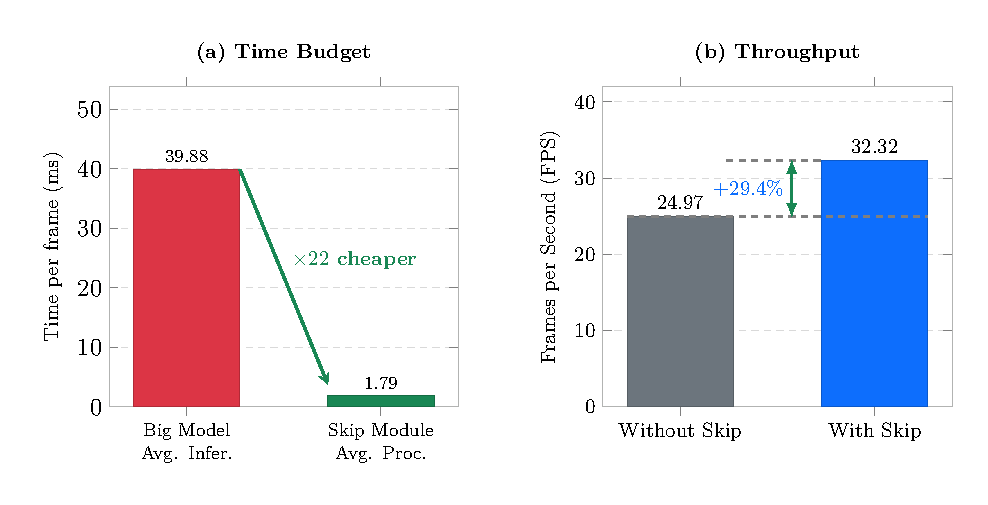
\includegraphics[width=\linewidth,keepaspectratio]{3.fig/fps_increase.pdf}
		\caption{Computational efficiency of the proposed skip module: (a)
			average processing time of the skip module (1.79~ms) compared to the
			BIG Model inference time (39.88~ms), representing a $\times 22$
			reduction; (b) system throughput with and without the skip module,
			yielding a 29.4\% improvement in FPS.}\label{fig:fps_increase}
	\end{figure}
	
	To evaluate the efficiency of the skip module, the BIG Model was run on
	the test set $\mathcal{D}_\text{test}$ with and without the skip
	module. The average processing time of the skip module, the BIG Model
	inference time, and the overall system FPS were recorded in both
	cases. The results are visualized in Fig.~\ref{fig:fps_increase}.
	
	As shown in Fig.~\ref{fig:fps_increase}, the skip module requires an
	average processing time of only 1.79~ms per frame, which is
	approximately $\times 22$ lower than the BIG Model inference time of
	39.88~ms. In the best case, the skip module correctly identifies and
	bypasses negative frames, contributing only 1.79~ms of overhead. In
	the worst case, where the skip module fails to bypass a frame and the
	BIG Model inference is subsequently invoked, the additional latency
	introduced by the skip module is 1.79~ms --- a mere 4.5\% increase
	relative to the BIG Model inference time. Overall, integrating the skip
	module improves system throughput by approximately 30\% on
	$\mathcal{D}_\text{test}$, demonstrating its effectiveness for
	real-time fire and smoke detection in indoor surveillance scenarios.
	
	\paragraph{Qualitative Analysis}\label{qualitative-analysis}
	
	To understand how the skip module operates in coordination with the
	BIG Model, we visualize the inference results of the
	\textsc{AccMotionDet} skip module on the test set
	$\mathcal{D}_\text{test}$ in RGB images together with the corresponding
	foreground motion masks generated by the skip module. The qualitative
	examples are organized into two major categories: success cases and
	failure cases.
	
	\textbf{Success Cases}
	
	\begin{figure}[t]
		\centering
		
\includegraphics[width=\linewidth,keepaspectratio]{3.fig/fig_qualitative_success.pdf}
		\caption{Qualitative results illustrating successful skip module
			operations. (a) and (b) Static background frames are correctly
			identified and skipped, avoiding unnecessary inference. (c) and (d)
			Frames containing active fire or smoke trigger the motion accumulator,
			correctly prompting the full deep learning model to evaluate the
			frame.}\label{fig:qualitative_success}
	\end{figure}
	
	Fig.~\ref{fig:qualitative_success} shows four representative success
	cases in which the skip module $\mathcal{S}$ operates as intended.
	These cases can be grouped into two categories:
	
	\begin{itemize}
		\item \textbf{Correctly skipped static background frames} (Fig.~\ref{fig:qualitative_success}a,b):
		\textsc{AccMotionDet} identifies static background frames and skips
		them without invoking the BIG Model. The corresponding motion masks are
		empty, indicating no active motion regions.
		\item \textbf{Correctly inferred fire/smoke frames} (Fig.~\ref{fig:qualitative_success}c,d):
		The module correctly detects active fire and smoke regions and
		forwards these frames for inference. The yellow boxes indicate
		motion-active blocks detected by \textsc{AccMotionDet}, which are
		concentrated in the fire/smoke regions, consistent with the continuous
		nature of these phenomena.
	\end{itemize}
	
	\textbf{Failure Cases}
	
	\begin{figure}[t]
		\centering
		
\includegraphics[width=\linewidth,keepaspectratio]{3.fig/fig_qualitative_failure.pdf}
		\caption{Qualitative analysis of skip module failure modes. (a) Missed
			detection: slow-developing or settled smoke fails to trigger the
			motion accumulator. (b--c) Wasted inferences: inaccurate motion
			detection or persistent motion (e.g., human activity) saturates the
			accumulator, preventing frame skipping. (d--e) Big Model error: frames
			are correctly passed to the deep learning model, yet the model
			produces incorrect predictions.}\label{fig:qualitative_failure}
	\end{figure}
	
	Fig.~\ref{fig:qualitative_failure} shows five representative failure
	cases, which can be grouped into three categories:
	
	\begin{itemize}
		\item \textbf{Wrongly skipped frames} (Fig.~\ref{fig:qualitative_failure}a):
		Slowly developing smoke or smoke in its settling phase produces motion
		that is too subtle to trigger the skip module, leading to missed
		detections.
		\item \textbf{Wrongly passed frames / wasted inference} (Fig.~\ref{fig:qualitative_failure}b,c):
		Noise or persistent non-fire motion prevents background frames from
		being skipped, resulting in unnecessary inference.
		\item \textbf{Incorrect BIG Model predictions} (Fig.~\ref{fig:qualitative_failure}d,e):
		Even when fire or smoke frames are correctly forwarded, the BIG Model
		may still produce an incorrect label, especially when the target
		objects (fire/smoke) occupy only a small portion of the frame.
	\end{itemize}
	
	\paragraph{Analysis of Eager Mode: Recall-FAR Trade-off}\label{sec:analysis_eager}
	
	\begin{figure}[t]
		\centering
		
\includegraphics[width=\linewidth]{3.fig/eager_timeline_success.png}
		\caption{A per-frame timeline example illustrating a recall-recovery
			scenario under \textsc{Eager} mode. Initially, the skip module
			suppresses inference on slow-developing smoke frames with minimal
			inter-frame motion (\textsc{Normal} Mode Zone). Once the classifier
			$\mathcal{M}$ yields positive predictions on $W_{\text{fire}}=1$
			consecutive frame(s) in \textsc{Normal} mode, the system transitions to
			\textsc{Eager} mode. This forces inference on every subsequent frame,
			enabling continuous smoke detection that would otherwise be missed---
			thus achieving a successful recall-recovery. Notably, from frames 163
			to 168, the system returns \texttt{None} predictions yet remains in
			\textsc{Eager} mode because the number of consecutive negative frames
			has not reached $W_{\text{clr}}=7$, which is insufficient to trigger an
			exit back to \textsc{Normal} mode.}\label{fig:eager_analysis_success}
	\end{figure}
	
	\begin{figure}[t]
		\centering
		
\includegraphics[width=\linewidth]{3.fig/eager_timeline_failure.png}
		\caption{A per-frame timeline example illustrating a false-alarm
			scenario under \textsc{Eager} mode. Once the classifier $\mathcal{M}$
			produces consecutive positive predictions over multiple frames on a
			static, false-alarm-prone scene, the system enters \textsc{Eager} mode
			and persists in it, forcing inference on every subsequent frame and
			causing an increase in FAR.}\label{fig:eager_analysis_failure}
	\end{figure}
	
	To demonstrate how \textsc{Eager} mode operates in practice, we
	visualize per-frame timeline results for both \textsc{Eager} and
	\textsc{Normal} mode on two representative videos: a success case
	(Fig.~\ref{fig:eager_analysis_success}) and a failure case
	(Fig.~\ref{fig:eager_analysis_failure}).
	
	As shown in Fig.~\ref{fig:eager_analysis_success}, \textsc{Eager} mode
	forces inference on frames that would otherwise be skipped due to
	insufficient motion, enabling detection of slow-developing or nearly
	stationary smoke that \textsc{Normal} mode alone would miss --- thus
	recovering recall in this critical scenario. However, a trade-off of
	\textsc{Eager} mode is an increase in the false alarm rate (FAR) from
	0.136\% to 0.251\% (Table~\ref{tb:cmp_other_temp_eager}). This arises
	because \textsc{Eager} mode cannot distinguish static, false-alarm-prone
	scenes from genuine slow-developing or nearly stationary smoke, as both
	exhibit near-zero inter-frame motion. On such scenes, consecutive
	positive predictions from $\mathcal{M}$ cause the system to enter and
	persist in \textsc{Eager} mode, sustaining forced inference and
	elevated FAR throughout the video, as illustrated in
	Fig.~\ref{fig:eager_analysis_failure}.
	
	This highlights a fundamental limitation of heuristic, motion-based
	skip logic: it is insufficient to robustly handle all scenarios. We
	leave this as an open research question, with potential directions
	including skip modules that incorporate richer cues (such as color,
	texture, or learned features) to discriminate between these scene
	types.
	
	\section{Conclusion}\label{sec:conclusion}
	
	We propose a lightweight, plug-and-play skip module $\mathcal{S}$
	designed to accelerate real-time fire and smoke detection in indoor
	surveillance scenarios. Operating at a negligible fraction
	(${\approx}4.5\%$) of the computational cost of the DL classifier
	$\mathcal{M}$, the skip module $\mathcal{S}$ efficiently filters out
	static background frames before they reach $\mathcal{M}$, reducing
	unnecessary inference overhead. Experiments on a real-world video
	dataset demonstrate that the proposed approach achieves approximately
	30\% throughput improvement while sustaining high detection recall,
	with a recall drop of only 1.23\% relative to the baseline. When
	augmented with \textsc{Eager} mode, the recall drop is further reduced
	to 0.05\%, nearly fully recovering baseline performance.
	
	Nevertheless, the proposed approach has certain limitations. First, the
	skip module $\mathcal{S}$ relies solely on inter-frame motion cues,
	which may be unsuitable for outdoor surveillance scenarios where
	persistent motion sources --- such as swaying vegetation, moving
	vehicles, etc. --- are continuously present, potentially causing
	$\mathcal{S}$ to pass the majority of frames to $\mathcal{M}$ and
	negating the efficiency gain. Second, the hyperparameters of
	$\mathcal{S}$ require dataset-specific tuning prior to deployment,
	incurring additional optimization overhead. Third, the overall
	detection accuracy of the system remains bounded by the capacity of
	$\mathcal{M}$, which is treated as a fixed component and not optimized
	in this work.
	
	Future work may explore alternative skip strategies --- such as
	leveraging color, texture, or learned features as gating cues --- and
	extend the framework to outdoor surveillance scenarios where
	motion-based filtering is less effective. Additionally, designing a
	hyperparameter-free or self-adaptive skip module, as well as jointly
	optimizing the skip module and the classifier in an end-to-end training
	framework, represent promising directions for further improving system
	efficiency and detection accuracy.
	
	%% Loading bibliography style file
	\bibliographystyle{cas-model2-names}
	
	% NOTE: rename/point this to the actual bib file provided by the user
	% (ref.bib / ref-3.bib) so that BibTeX can resolve all \citep/\citet keys.
	\bibliography{refs.bib}

    % ---------------------------------------------------------------------
% Author biographies (cas-dc \bio ... \endbio format)
% Converted from 7bio.tex (IEEEbiography) to match the style used in the
% original B-2.tex template.
% ---------------------------------------------------------------------

\bio{figs/authors/a1}
Van-Ha Hoang received an engineering degree in Software and an M.S.
degree in Computer Science from the University of Information
Technology (UIT), VNUHCM, in 2014 and 2018, respectively. He is
currently pursuing his Ph.D. degree in the Department of Software at
Sejong University. In 2018, he was an internship student at the
National Institute of Informatics (NII) in Tokyo, Japan. His research
interests include computer vision and deep learning.
\endbio

\bio{figs/authors/a2}
Jong Weon Lee received an M.S. degree in Electrical and Computer
Engineering from the University of Wisconsin at Madison in 1991, and a
Ph.D. degree from the University of Southern California in 2002. He is
presently a Professor in the Department of Software at Sejong
University. His research interests include virtual reality, augmented
reality, and human-computer interaction.
\endbio

\bio{figs/authors/a3}
Chun-Su Park received the B.S. and Ph.D. degrees in electrical
engineering from Korea University, Seoul, in 2003 and 2009,
respectively. From 2009 to 2010, he was a Visiting Scholar with the
Signal and Image Processing Institute, University of Southern
California, Los Angeles, CA, USA. From 2010 to 2012, he was a Senior
Research Engineer with Samsung Electronics. From 2012 to 2014, he was
an Assistant Professor with the Department of Information and
Telecommunication Engineering, Sangmyung University. From 2014 to 2016,
he was an Associate Professor with the Department of Digital Contents,
Sejong University. He joined the Department of Computer Education,
Sungkyunkwan University, in 2017, where he is currently an Associate
Professor. His research interests include video signal processing,
parallel computing, and multimedia communications.
\endbio
	
\end{document}
